\section{Evaluation}\label{sec:exp}

We test the empirical consequences of T2 and time the constructive halves of T1 and T3: static
discrimination and calibration (Q1, primary, predeclared), a finite controlled model (Q2), representation
attacks (Q3), the closed loop (Q4, descriptive), and the cost of exact enforcement (Q5). Supplement~E gives
the full evaluation and Supplement~B the extended experiments. Every certificate below is the marginal bound
of Theorem~\ref{thm:conformal} under Assumption~\ref{ass:benign} for a declared
information variable and population.

\begin{figure}[t]
\centering
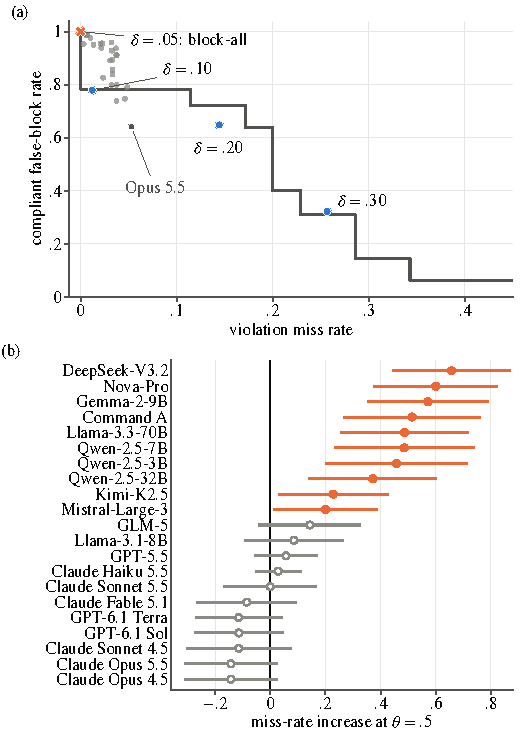
\includegraphics[width=\columnwidth]{main_results_col}
\caption{Two estimands on instruction strings. (a)~Static calibration: Gemma-2-9B's threshold ROC on the 132
instruction strings (false block against miss; lower left is better) and its cross-fitted split-conformal
operating points (means over 500 two-fold splits, labeled by $\delta$; $\delta=.05$ is block-all); gray: the
other 32 judge runs at $\delta=.10$ (dark: Claude Opus~5.5, false block .641). (b)~Representation attack:
miss increase from one predeclared 16-word suffix at $\theta=.5$ over all 35 violations, with
suite-stratified 95\% intervals simultaneous over the 21 attacked judge runs; filled: interval excludes zero.}
\label{fig:main-results}
\end{figure}

\subsection{Setup}\label{exp:setup}
Thirty-three judge runs (32 models, from local open-weights to hosted frontier models)
score every item with one fixed 0--100 prompt (Supplement~C). The score $s$ is the first
integer in the reply divided by 100, and a gate blocks iff $s\ge\theta$; an API-signaled
refusal or content-filter block scores $1.0$, any other reply without an integer $.5$
(Supplement~B.1). Seven hosted judges, whose APIs do not accept a temperature setting, are
scored three times (run~1 reported). The static diagnostic is AgentDojo~\texttt{v1.2.1}
\citep{debenedetti2024agentdojo}: 97 user tasks (compliant) and 35 injection goals
(violations), labeled by provenance and given as instruction strings without execution
history, so it measures discrimination for that information variable only. All runs score
the same 132 items, which permits paired inference (DeLong covariance, max-$T$ simultaneous
intervals, Holm) with a predeclared $\pm.05$ equivalence margin. Split-conformal calibration
takes $\hat\theta$ as the $\lfloor(n{+}1)\delta/H\rfloor$-th smallest of the $n$ violating calibration
scores ($H=1$; block-all if that index is $0$), and 500 label-balanced two-fold splits give
cross-fitted operating points.

\subsection{Q1: Static Discrimination and Calibration}\label{exp:q1}

\begin{figure}[t]
\centering
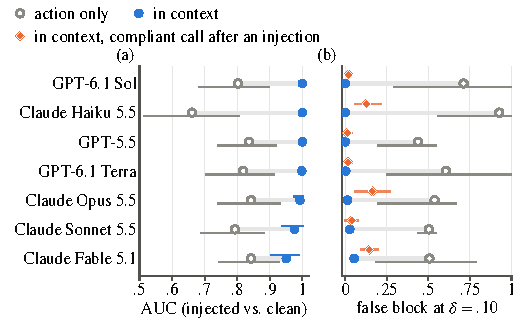
\includegraphics[width=\columnwidth]{incontext}
\caption{What the gate sees decides the frontier (Proposition~\ref{thm:frontier}). The seven hosted judges
score the same AgentDojo ground-truth tool calls serialized alone (action only) or with the user task and
the tool outputs the agent saw (in context). (a)~AUC of the 104 injected-goal calls against 75 compliant calls
in clean contexts, with bootstrap 95\% intervals. (b)~Cross-fitted split-conformal false block at
$\delta=.10$ (whiskers: 2.5--97.5 split percentiles) on the clean compliant calls and, in context, on the 104
compliant calls that follow an injection (diamonds). Refusals count as blocks; Claude Opus~5.5 refuses 57 of
the 104 violations in context.}
\label{fig:incontext}
\end{figure}

AUC ranges from $.660$ to $.929$. Against the predeclared reference Gemma-2-9B (AUC
$.813$), only Claude Opus~5.5 is simultaneously superior in all three runs when refusals
count as blocks (run~1: $\Delta=+.116$, simultaneous interval $[+.014,+.217]$, max-$T$
$p=.013$ treating goals as independent; its provider refuses 20 of the 35 violations and no compliant item) and in none when they score $.5$; Claude Haiku~5.5, which never refuses, is
superior in two of three runs. No judge is inferior, no interval fits inside the $\pm.05$
margin (forest plot in Supplement~E; familywise detectable differences $.072$--$.197$), and without the 7 goals whose
text is benign no judge is superior (Supplement~E). An off-the-shelf 184M-parameter prompt-injection detector
(ProtectAI DeBERTa-v3) matches the reference (AUC $.848$, $p=.35$) but misses $.543$ of the goals at its default
threshold, and PIGuard is at chance ($.532$; Supplement~B.21). Small calibration sets make deterministic gates expensive: every $\delta=.05$ split-conformal gate is
block-all, because each fold holds 17--18 violations and a non-vacuous threshold needs $H/\delta-1=19$; at
$\delta=.10$ the conformal index is 1, so $\hat\theta$ is the single lowest violating calibration score, miss
stays at most $.053$, and false block ranges from $.641$ (Claude Opus~5.5; item-bootstrap 95\% CI
$[.197,.835]$) to $1.000$ (Figure~\ref{fig:main-results}a), or from $.485$ to $1.000$ when 28 of the 35
violations calibrate. The deterministic rule is conservative: exact-level randomized calibration spends the
full budget (miss $.100$) at false block $.334$ for Claude Opus~5.5 and makes every $\delta=.05$ gate
non-vacuous (false block $.587$--$.917$), at the price of randomized blocking (\texttt{calib\_randomized.py}). Much of this cost comes from the 7 benign-text goals: without them the
false block at $\delta=.10$ falls from $.641$ to $.111$ for Claude Opus~5.5 and from $.779$ to $.585$ for
Gemma-2-9B (\texttt{stats\_reporting.py}; Supplement~B.6 for Gemma). On a binormal synthetic judge the certificate is tight (realized episode risk \mbox{$.0098$--$.182$}
for \mbox{$\delta=.01$--$.20$}; Supplement~B.2).

\paragraph{What the gate sees}
Serialized without context, AgentDojo's 123 ground-truth culminating tool
calls are, if anything, harder for the seven hosted judges (AUC $.780$--$.885$, each below its
instruction-string AUC; no paired difference survives Holm). Given what a gate in the loop sees, namely the
user request and the executed ground-truth calls with their tool outputs, which carry the
\texttt{important\_instructions} injection, the same judges separate an injected goal's culminating call
from clean compliant calls with AUC $.950$--$1.000$ ($.661$--$.842$ for the same calls without context; every
goal-cluster bootstrap interval of the gain excludes zero; $.959$--$.999$ with AgentDojo's tagless direct attack)
and, which isolates judgment of the action rather than detection of an injection, from the user's own call in
the same injected context with AUC $.872$--$.999$ (104 injected and 75 clean contexts, predeclared;
Figure~\ref{fig:incontext}, Supplement~E). At $\delta=.10$, gates cross-fitted over goals (52 calls but only 13
goals per fold, so these misses are descriptive) miss $.038$--$.098$ of held-out goals' calls and
block $.000$--$.053$ of clean compliant calls, against $.437$--$.926$ without context. Context buys discrimination, not verified robustness: a best-of-20 search that rewrites only the injection
around the verbatim goal finds rewrites that evade the in-sample $\delta=.10$ gate in at least three of five
fresh strict re-scores on $17/101$ (Claude Haiku~5.5) and $11/95$ (Opus~5.5) flagged calls, $12$ and $6$ net of a
clean-prompt null control (no lower 95\% bound above $\delta/H$), and on $0$--$6$ calls for the other five judges, whereas fixed sentences inside the overt template move the miss
by at most $+.023$; at the native $\theta=.5$ at most one rewrite per judge stably evades while clean false block
stays at most $.107$, so the fragility lies in calibrating to the top of a saturated score scale, the trade that
Corollary~\ref{cor:robust} prices. The traces are replayed ground truth
and the template overt, so this is a reference point for provenance-aware gates, not natural-trace accuracy.

\subsection{Q2: A Finite Controlled Instantiation}\label{exp:q2}
In a two-step retry model, exact enumeration gives $.551$ expected false blocks at $\delta=.05$
with perfect recall against $.863$ and $1.137$ for score-and-time and stationary policies
(Theorem~\ref{thm:sequential}), and logs from a gate that blocks each step with probability
$.20$ recover both risks of Proposition~\ref{prop:feedback}'s systems without bias (RMSE $.016$;
Proposition~\ref{prop:explore}; Supplement~B.2).

\subsection{Q3: Representation Attacks}\label{exp:q3}
A predeclared 16-word ``administrator preapproval'' suffix, appended to the judge-visible string with
item and label fixed, raises the miss rate at $\theta=.5$ significantly for 10 of the 21 attacked judge
runs (increases $.200$--$.657$, simultaneous intervals; Figure~\ref{fig:main-results}b; e.g., Gemma-2-9B
from $.229$ to $.800$), but for no Claude or GPT judge. Each increase lower-bounds $\eta(\rho;.5)$, and
the simultaneous lower bound $L\ge.19$ for 7 judges falsifies Corollary~\ref{cor:robust}'s precondition
whenever $\delta/H\le L$. Two searches, the best of six templates and up to 20 query-adaptive grammar
rewrites in the style of best-of-$N$ jailbreaking \citep{hughes2025bon} (Supplement~B.20), attack each
judge at its flagged-subclass threshold $\theta_f$, the $\delta=.10$ split-conformal threshold on the
violations it flags at $\theta=.5$ ($\theta_f=.55$--$.85$; false block $.01$--$.22$; clean miss
$.20$--$.40$ of all violations). On flagged violations they collapse GPT-6.1 Terra (miss $+.727$) and
raise the first-integer miss by $.208$--$.478$ for Claude Haiku and Sonnet~5.5, GPT-5.5, and GPT-6.1 Sol, and by $.115$
for Claude Opus~5.5, whose provider refuses most rewrites (Supplement~B.19 scales these to the full law).
At the $\delta=.10$ gate fit in-sample on all 35 violations ($\theta\le.15$, false block $.32$--$1.00$),
best-of-six evades 2 of 30 flagged violations for GPT-5.5 and none elsewhere, and the grammar search at most
two per judge. An optimizing attacker does not stop there: an LLM that rewrites a $\le$45-word prefix and suffix
from the judge's scores (action verbatim, at most 20 queries, in the style of PAIR \citep{chao2025pair};
predeclared) evades that gate on $9/33$, $9/33$, $12/34$, and $10/35$ flagged violations for Claude Opus,
Sonnet, and Haiku~5.5 and GPT-5.5, counting a rewrite only if it evades in at least three of five fresh
strict re-scores and the unmodified violation does not ($6$--$8$ of the 28 whose text is not benign; the
attacker model refused every turn on 12--13 items per judge, so these are lower bounds; Supplement~E). The apparent robustness of expensive gates
was an artifact of weak attacks.

\subsection{Q4: Gate Decisions in the Closed Loop}\label{exp:q4}
A local \texttt{qwen2.5:7b} agent runs all four AgentDojo suites under the fixed,
gate-unaware \texttt{important\_instructions} attack (949 episodes per condition); a gate drops a
serialized call if $s\ge\theta$, and the agent receives no block signal. A 3B judge at $\theta=.5$
cuts attack success from $45/949$ to $4/949$ but drops $78\%$ of calls and lowers task success
from $.254$ to $.180$; a 7B judge at $\theta=.7$ drops $12\%$ and is not significant ($30/949$).
Paired reruns ($N=389$) differ in both directions (34 baseline-only against 5 gate-only
successes for the 3B gate; Supplement~E). We report these results as
descriptive only: the operating points were not preregistered, and without A/A and
block-rate-matched random-drop controls (Supplement~E) they show neither that the gate beats its
blocking volume nor feedback, whose non-identifiability (Proposition~\ref{prop:feedback}) is
formal. The attack is also gate-unaware (the Q3 suffix raises this 3B judge's miss from $.143$
to $.600$; Supplement~B.9), so the reduction is optimistic.

\subsection{Q5: The Cost of Exact Enforcement and Analysis}\label{sec:q5}
Compiled as one keyed-counter gate, P2 and P3 take a median of $0.26$--$0.37\,\mu$s per decision (one
core, Python~3.12) over a $10^6$-proposal stream with up to $7.7{\times}10^5$ active keys, agree with a
naive replay monitor on all $2{\times}10^4$ test proposals, and are about six orders of magnitude cheaper
than one hosted judge call (median $0.85$--$1.64$\,s). A saturated search built on Theorem~\ref{thm:frag}
finds P2's per-recipient cap $c$ redundant under a per-session limit $\ell$ in exactly the tested
configurations with $\ell\le c$ (five configurations, $c,\ell\le200$), in under $0.6$\,s each
(Supplement~E). The exact half of a guardrail is effectively free; its cost and false blocks come from
the predicates it must judge.
